% ============================================================
%  يُترجَم بـ XeLaTeX  (في Overleaf: Menu → Compiler → XeLaTeX)
%  الخط: Amiri (متوفر في Overleaf، أو حمّله من github.com/aliftype/amiri)
% ============================================================
\documentclass[12pt,a4paper]{article}
\usepackage[a4paper,margin=1.2cm,top=2.3cm,bottom=2.9cm,headheight=15pt,footskip=1.5cm]{geometry}
\usepackage{amsmath,amssymb}
\usepackage{icomma}
\usepackage[english,bidi=default,layout=lists]{babel}
\babelprovide[import,main]{arabic}
\babelfont{rm}[Scale=1.08]{Amiri}
\babelfont{sf}[Scale=1.08]{Amiri}
\usepackage[most]{tcolorbox}
\usepackage{tikz}
\usetikzlibrary{arrows.meta,calc,shadings}
\usepackage{array}
\usepackage{colortbl}
\usepackage{fancyhdr}
\usepackage{titlesec}
\usepackage{enumitem}
\usepackage{collcell}
\usepackage{needspace}
\usepackage{etoolbox}
\newcolumntype{C}{>{\collectcell\ar}c<{\endcollectcell}}
\pretocmd{\section}{\Needspace{15\baselineskip}}{}{}
\pretocmd{\subsection}{\Needspace{11\baselineskip}}{}{}

\definecolor{cDef}{HTML}{1F4E9C}
\definecolor{cThm}{HTML}{B3261E}
\definecolor{cRem}{HTML}{2E7D32}
\definecolor{cEx}{HTML}{C76B00}
\definecolor{cMeth}{HTML}{6A1B9A}
\definecolor{cSol}{HTML}{00695C}
\definecolor{cSec}{HTML}{1F3A68}

\titleformat{\section}{\Large\bfseries\color{cSec}}{\thesection.}{0.6em}{}[{\color{cSec!60}\titlerule[1pt]}]
\titleformat{\subsection}{\large\bfseries\color{cThm!85!black}}{\thesubsection.}{0.5em}{}
\titlespacing*{\section}{0pt}{14pt}{8pt}
\titlespacing*{\subsection}{0pt}{10pt}{5pt}
\setlength{\parindent}{0pt}
\setlength{\parskip}{4pt}
\setlist{itemsep=2pt,topsep=3pt}

\newtcolorbox{arbox}[3][]{enhanced,
  colback=#2!5,colframe=#2!80!black,arc=2mm,boxrule=0.8pt,
  left=6pt,right=6pt,top=8pt,bottom=5pt,
  fonttitle=\bfseries,coltitle=white,
  title={\foreignlanguage{arabic}{#3}},
  attach boxed title to top right={xshift=-5mm,yshift=-3mm},
  boxed title style={colback=#2!80!black,arc=1.5mm,boxrule=0pt},
  before upper={\selectlanguage{arabic}},
  before skip=8pt,after skip=8pt,breakable,#1}
\newenvironment{BOX}[2]{\begin{otherlanguage}{english}\begin{arbox}{#1}{#2}}{\end{arbox}\end{otherlanguage}}
\newenvironment{tarif}[1][تعريف]{\begin{BOX}{cDef}{#1}}{\end{BOX}}
\newenvironment{khassia}[1][خاصية]{\begin{BOX}{cThm}{#1}}{\end{BOX}}
\newenvironment{molahada}[1][ملاحظة]{\begin{BOX}{cRem}{#1}}{\end{BOX}}
\newenvironment{mithal}[1][مثال]{\begin{BOX}{cEx}{#1}}{\end{BOX}}
\newenvironment{tariqa}[1][طريقة]{\begin{BOX}{cMeth}{#1}}{\end{BOX}}

\newcounter{exo}
\newenvironment{tamrin}[1]{\stepcounter{exo}\begin{BOX}{cSec}{التمرين \theexo: #1}}{\end{BOX}}
\newenvironment{hal}{\Needspace{12\baselineskip}\begin{otherlanguage}{english}\begin{arbox}[breakable]{cSol}{حل التمرين \theexo}}{\end{arbox}\end{otherlanguage}}

\newenvironment{LTR}{\begin{otherlanguage}{english}}{\end{otherlanguage}}
\newcommand{\ar}[1]{\foreignlanguage{arabic}{#1}}

\renewcommand{\dots}{\mathinner{\ldotp\ldotp\ldotp}}
\renewcommand{\ldots}{\mathinner{\ldotp\ldotp\ldotp}}
\renewcommand{\cdots}{\mathinner{\cdotp\cdotp\cdotp}}
\newcommand{\N}{\mathbb{N}}
\newcommand{\Z}{\mathbb{Z}}
\newcommand{\D}{\mathbb{D}}
\newcommand{\Q}{\mathbb{Q}}
\newcommand{\R}{\mathbb{R}}
\newcommand{\pgcd}{\operatorname{PGCD}}
\newcommand{\ppcm}{\operatorname{PPCM}}

% \NLseg{a}{b}{[}{]} ; \NLright{a}{[} ; \NLleft{b}{]}  (interval on a number line)
\newcommand{\NLseg}[4]{\begin{LTR}\begin{tikzpicture}[baseline=-0.6ex]
 \draw[-{Stealth[length=2mm]},gray!70](0,0)--(3.4,0);
 \draw[line width=2pt,cThm!80!black](0.7,0)--(2.7,0);
 \node[cThm!80!black,font=\LARGE] at (0.7,0){$#3$};
 \node[cThm!80!black,font=\LARGE] at (2.7,0){$#4$};
 \node[below=3pt,font=\footnotesize] at (0.7,0){$#1$};
 \node[below=3pt,font=\footnotesize] at (2.7,0){$#2$};
\end{tikzpicture}\end{LTR}}
\newcommand{\NLright}[2]{\begin{LTR}\begin{tikzpicture}[baseline=-0.6ex]
 \draw[-{Stealth[length=2mm]},gray!70](0,0)--(3.4,0);
 \draw[line width=2pt,cThm!80!black](1.3,0)--(3.3,0);
 \node[cThm!80!black,font=\LARGE] at (1.3,0){$#2$};
 \node[below=3pt,font=\footnotesize] at (1.3,0){$#1$};
\end{tikzpicture}\end{LTR}}
\newcommand{\NLleft}[2]{\begin{LTR}\begin{tikzpicture}[baseline=-0.6ex]
 \draw[-{Stealth[length=2mm]},gray!70](0,0)--(3.4,0);
 \draw[line width=2pt,cThm!80!black](0.05,0)--(2.1,0);
 \node[cThm!80!black,font=\LARGE] at (2.1,0){$#2$};
 \node[below=3pt,font=\footnotesize] at (2.1,0){$#1$};
\end{tikzpicture}\end{LTR}}

% ---------- social-media icons (pure TikZ) ----------
\definecolor{cFB}{HTML}{1877F2}
\definecolor{cTG}{HTML}{229ED9}
\definecolor{cIG1}{HTML}{FEDA75}
\definecolor{cIG2}{HTML}{D62976}
\definecolor{cIG3}{HTML}{4F5BD5}
\newcommand{\fbicon}{\begin{LTR}\begin{tikzpicture}[baseline=-0.75ex,x=1em,y=1em]
 \fill[cFB] (0,0) circle (0.55);
 \node[white,inner sep=0,font=\usefont{TU}{lmss}{bx}{n}\small] at (0.04,-0.02) {f};
\end{tikzpicture}\end{LTR}}
\newcommand{\igicon}{\begin{LTR}
\begin{tikzpicture}[baseline=-0.75ex,x=1em,y=1em]
 \shade[lower left=cIG1,lower right=cIG2,upper left=cIG2,upper right=cIG3,rounded corners=0.28em] (-0.55,-0.55) rectangle (0.55,0.55);
 \draw[white,line width=0.09em,rounded corners=0.18em] (-0.36,-0.36) rectangle (0.36,0.36);
 \draw[white,line width=0.09em] (0,0) circle (0.17);
 \fill[white] (0.22,0.22) circle (0.05);
\end{tikzpicture}\end{LTR}}
\newcommand{\tgicon}{\begin{LTR}
\begin{tikzpicture}[baseline=-0.75ex,x=1em,y=1em]
 \fill[cTG] (0,0) circle (0.55);
 \fill[white] (-0.33,0.0) -- (0.32,0.27) -- (0.2,-0.3) -- (0.0,-0.15) -- (-0.08,-0.28) -- (-0.08,-0.08) -- cycle;
 \fill[cTG!70!black] (-0.08,-0.08) -- (0.25,0.2) -- (0.0,-0.15) -- (-0.08,-0.28) -- cycle;
\end{tikzpicture}\end{LTR}}
% page number: black box, white two-digit number, at the right of the social row
\newcommand{\PageBox}{\begin{LTR}\tikz[baseline=(p.base)]\node[fill=black,text=white,inner sep=2.5pt,minimum width=1.6em,minimum height=1.3em,font=\usefont{TU}{lmss}{bx}{n}\small](p){\ifnum\value{page}<10 0\fi\arabic{page}};\end{LTR}}
% visual left-to-right order: Telegram | Instagram | Facebook | page box
\newcommand{\SocialRow}{\begin{otherlanguage}{english}%
 \ar{\textbf{الأستاذ سوايسية هشام للرياضيات}}\ \tgicon\hfill
 \textbf{prof\_hicham\_math}\ \igicon\hfill
 \ar{\textbf{الأستاذ سوايسية هشام للرياضيات}}\ \fbicon\hspace{2.2em}\PageBox\end{otherlanguage}}

\pagestyle{fancy}
\fancyhf{}
\renewcommand{\headrulewidth}{0.6pt}
\renewcommand{\footrulewidth}{0.4pt}
% \SetHeader{right head: document title}{left head: level -- stream}
\newcommand{\SetHeader}[2]{%
 \fancyhead[C]{\parbox{\textwidth}{\ar{#1\hfill #2}}}%
 \fancyfoot[C]{\parbox{\textwidth}{\small\SocialRow}}}
\usepackage{tkz-tab}
\usepackage{multicol}
% variation / sign table (LTR)
\newenvironment{TAB}{\par\begin{center}\begin{LTR}\begin{tikzpicture}[scale=0.95,every node/.style={font=\small}]}{\end{tikzpicture}\end{LTR}\end{center}}
% grid + axes, clipped: \begin{GR}{xmin}{xmax}{ymin}{ymax}{unit cm}
\newenvironment{GR}[5]{\par\begin{center}\begin{LTR}\begin{tikzpicture}[x=#5cm,y=#5cm,font=\footnotesize]
 \draw[gray!25,very thin] (#1,#3) grid (#2,#4);
 \draw[-{Stealth[length=2mm]}] (#1,0)--(#2+0.3,0) node[below left]{$x$};
 \draw[-{Stealth[length=2mm]}] (0,#3)--(0,#4+0.3) node[below left]{$y$};
 \node[below left] at (0,0){$O$};
 \begin{scope}\clip (#1,#3) rectangle (#2,#4);}
{\end{scope}\end{tikzpicture}\end{LTR}\end{center}}
\newcommand{\Ticks}[2]{\foreach \t in {#1} \node[below,font=\scriptsize] at (\t,0){$\t$}; \foreach \t in {#2} \node[left,font=\scriptsize] at (0,\t){$\t$};}
\newcommand{\bx}[1]{\ensuremath{\colorbox{cDef!12}{$\displaystyle #1$}}}
\newcommand{\TwoCol}[4]{\par\begin{LTR}\noindent\begin{minipage}[t]{#1\textwidth}\selectlanguage{arabic}#2\end{minipage}\hfill\begin{minipage}[t]{#3\textwidth}\selectlanguage{arabic}#4\end{minipage}\end{LTR}\par}
\newcommand{\RL}[4]{\TwoCol{#3}{#4}{#1}{#2}}  % \RL{w1}{right content}{w2}{left content}
\newcommand{\ok}{$\textcolor{cRem}{\checkmark}$}
\newcommand{\limn}{\displaystyle\lim_{n\to+\infty}}
% sub-questions, each on its own line
\newenvironment{sq}{\begin{itemize}[leftmargin=2.4em,itemsep=3pt]}{\end{itemize}}
\newcommand{\qa}{\item[(أ)]}\newcommand{\qb}{\item[(ب)]}\newcommand{\qc}{\item[(جـ)]}\newcommand{\qd}{\item[(د)]}\newcommand{\qe}{\item[(هـ)]}
\newcommand{\pa}{\par\smallskip\textbf{(أ)} }\newcommand{\pb}{\par\smallskip\textbf{(ب)} }\newcommand{\pc}{\par\smallskip\textbf{(جـ)} }\newcommand{\pd}{\par\smallskip\textbf{(د)} }\newcommand{\pe}{\par\smallskip\textbf{(هـ)} }
\newcommand{\QQ}[1]{\par\smallskip\textbf{#1.} }
\newenvironment{tmr}{\stepcounter{exo}\begin{BOX}{cSec}{تمرين محلول \theexo}}{\end{BOX}}
\newcommand{\ABC}[3]{\\[2pt]\begin{tabular}{p{0.28\textwidth}p{0.28\textwidth}p{0.28\textwidth}}(جـ) \ #3 & (ب) \ #2 & (أ) \ #1\end{tabular}}
\pretocmd{\section}{\Needspace{24\baselineskip}}{}{}
\newtcbox{\bxtbox}{on line,colback=cDef!12,colframe=cDef!12,boxrule=0pt,arc=1pt,boxsep=0pt,left=2pt,right=2pt,top=1pt,bottom=1pt}
\newcommand{\bxt}[1]{\foreignlanguage{english}{\bxtbox{\ar{#1}}}}
\usepackage{longtable}
\setlength{\LTpre}{4pt}\setlength{\LTpost}{0pt}
\newcommand{\Phase}[1]{\textbf{#1}}
\newcommand{\Fld}[2]{\textbf{#1:}\ #2}
% رأس المذكرة على نمط النموذج: إطار بعنوان «مذكرة رقم»، معلومات الحصة، ثم إطار الكفاءات
\newcommand{\ModhHead}[9]{%
\begin{LTR}
\begin{tcolorbox}[enhanced,colback=white,colframe=cThm!85!black,arc=4mm,boxrule=1pt,top=14pt,bottom=6pt,left=8pt,right=8pt,
 overlay={\node[fill=cThm!85!black,text=white,rounded corners=3mm,inner xsep=14pt,inner ysep=4pt,font=\large\bfseries] at ([yshift=0pt]frame.north){\ar{مذكرة رقم #1}};},
 before upper={\selectlanguage{arabic}}]
\begin{tabular}{@{}p{0.4\linewidth}p{0.55\linewidth}@{}}
\Fld{المستوى}{#2} & \Fld{الثانوية}{\dotfill}\\[3pt]
\Fld{المادة}{رياضيات} & \Fld{ميدان التعلم}{#3}\\[3pt]
\Fld{المدة}{#5} & \Fld{الوحدة التعلمية}{#4}\\[3pt]
\Fld{الأستاذ}{\dotfill} & \Fld{المحتوى المعرفي}{#6}\\
\end{tabular}
\end{tcolorbox}
\begin{tcolorbox}[enhanced,colback=white,colframe=cThm!85!black,arc=3mm,boxrule=0.8pt,sidebyside,sidebyside align=top,lefthand ratio=0.5,
 segmentation style={dashed,cThm!60},before upper={\selectlanguage{arabic}},before lower={\selectlanguage{arabic}}]
\textbf{الكفاءات المستهدفة:}\par #8
\tcblower
\textbf{الكفاءات القبلية:}\par #7
\end{tcolorbox}
\end{LTR}
\par\smallskip\textbf{الوسائل:} #9\par\smallskip}
\newenvironment{Sayr}{%
\begin{LTR}\renewcommand{\arraystretch}{1.25}\setlength{\tabcolsep}{4pt}\relpenalty=10000\binoppenalty=10000\tolerance=9000\emergencystretch=0.3\linewidth
\begin{longtable}{|p{0.09\textwidth}|>{\centering\arraybackslash}p{0.05\textwidth}|p{0.71\textwidth}|>{\centering\arraybackslash}p{0.09\textwidth}|}
\hline\rowcolor{cThm!12}\ar{\footnotesize\textbf{توجيهات وتعاليق}} & \ar{\footnotesize\textbf{المدة}} & \ar{\textbf{سير الحصة}} & \ar{\footnotesize\textbf{مراحل الحصة}}\\\hline\endhead
\hline\endfoot}{\end{longtable}\end{LTR}}
% سطر في الجدول: \Row{مرحلة}{سير}{مدة}{توجيهات}
\newcommand{\Row}[4]{\ar{\small #4} & \ar{#3} & \ar{#2} & \cellcolor{cThm!8}\ar{\Phase{#1}}\\\hline}

\newcommand{\Lab}[2]{\foreignlanguage{english}{\tcbox[on line,colback=#1,colframe=#1,boxrule=0pt,arc=2pt,boxsep=1pt,left=5pt,right=5pt,top=1pt,bottom=1pt]{\ar{\textcolor{white}{\textbf{#2}}}}}}
\newcommand{\Num}[1]{\foreignlanguage{english}{\tikz[baseline=(c.base)]\node[fill=cDef,text=white,inner sep=2pt,font=\footnotesize\bfseries](c){#1};}}
\newcommand{\ck}{\ensuremath{{\color{cRem}\checkmark}}}
\newenvironment{Kad}[1]{\par\smallskip\Lab{#1}}{\par}
\newcommand{\RR}[1]{\ifmmode{\color{cThm}#1}\else$\mbox{\color{cThm}#1}$\fi}
\newcommand{\T}[1]{$\mbox{\color{cDef}\bfseries #1}$}
\SetHeader{\small\bfseries\color{cSec}مذكرات محور: الدالة الأسية}{\small\color{cSec}السنة الثالثة ثانوي -- تسيير واقتصاد}
\begin{document}
\begin{LTR}
\begin{tcolorbox}[enhanced,colback=cThm!85!black,colframe=cThm!85!black,arc=3mm,halign=center,boxrule=0pt,top=12pt,bottom=12pt,before upper={\selectlanguage{arabic}}]
{\color{white}\fontsize{24}{30}\selectfont\bfseries مذكرات محور: الدالة الأسية}\\[8pt]
{\color{white}\large السنة الثالثة ثانوي -- تسيير واقتصاد}\\[4pt]
{\color{white}\large 6 مذكرات (12 ساعة) -- السنة الدراسية 2026-2027}
\end{tcolorbox}
\end{LTR}
\begin{BOX}{cThm}{يتضمن هذا العمل}
\begin{enumerate}[label=\textbf{مذكرة \arabic{enumi}:},leftmargin=6em,start=34]
\item الدالة الأسية: التعريف ، الخواص ، الدراسة.
\item معادلات ومتراجحات تتضمن أسيات.
\item النهايات الشهيرة والتزايد المقارن ، دوال $e^u$.
\item الدالة الأسية ذات الأساس $a$ ، الدوال القوى.
\item مشكلات إيداع وتسديد.
\item مسائل حول دراسة دوال لوغاريتمية وأسية.
\end{enumerate}
الحلول مفصّلة: المعطيات بالأسود ، \T{العناوين} و\RR{النتائج} بلون مختلف ، وكل سؤال في سطر.
\end{BOX}
\newpage
\ModhHead{34}{3 ت ا}{تحليل}{الدالة الأسية}{02 سا}{الدالة الأسية النيبيرية: التعريف ، الخواص ، الدراسة}%
{\begin{itemize}\item الدالة $\ln$ ودراستها.\end{itemize}}%
{\begin{itemize}\item تعريف الدالة الأسية ومعرفة خواصها ، مشتقتها ، تمثيلها البياني وسلوكها التقاربي.\end{itemize}}%
{المنهاج ، الكتاب المدرسي ، الآلة الحاسبة العلمية والبيانية.}
\begin{Sayr}
\Row{مرحلة الانطلاق}{%
\textbf{التهيئة النفسية:} $\ln$ متزايدة تماماً من $-\infty$ إلى $+\infty$: هل لكل عدد $x$ عدد موجب $y$ يحقق $\ln y=x$ ؟}{10 د}{سؤال.}
\Row{التشخيص والاكتشاف}{%
\Lab{cEx}{مناقشة النشاط صفحة 150}\par\textbf{(1)} باستعمال جدول تغيرات $\ln$ ، بيّن أن المعادلة $\ln y=x$ تقبل حلاً وحيداً $y>0$ من أجل كل عدد حقيقي $x$.\par\textbf{(2)} احسب بالآلة الحاسبة الحلول من أجل $x=1$ ، $x=0$ ، $x=-1$.}{35 د}{الآلة الحاسبة.}
\Row{}{%
\Lab{cDef}{مناقشة النشاط}\par\textbf{(1)} $\ln$ مستمرة ومتزايدة تماماً على $]0;+\infty[$ ، وتأخذ كل القيم من $-\infty$ إلى $+\infty$: حسب مبرهنة القيم المتوسطة للمعادلة \RR{حل} \RR{وحيد} ، نرمز له بـ $e^x$.\par\textbf{(2)} $e^1\approx\RR{2{,}718}$ ؛ $e^0=\RR{1}$ ؛ $e^{-1}\approx\RR{0{,}368}$.}{}{}
\Row{بناء المعارف}{%
\Lab{cDef}{تعريف}\ من أجل كل عدد حقيقي $x$: $\RR{y=e^x}$ تكافئ $\RR{\ln y=x}$ مع $y>0$. ومنه: $e^x>0$ ، $\ln\left(e^x\right)=x$ ، و $e^{\ln x}=x$ من أجل $x>0$.}{50 د}{التناظر مع $\ln$.}
\Row{}{%
\Lab{cThm}{خاصية}\par\textbf{(1)} $\RR{e^{a+b}=e^ae^b}$ ؛ $\RR{e^{-a}=\dfrac1{e^a}}$ ؛ $\RR{e^{a-b}=\dfrac{e^a}{e^b}}$ ؛ $\RR{\left(e^a\right)^n=e^{na}}$.}{}{}
\Row{}{%
\Lab{cMeth}{البرهان}\ (الأولى) $\ln\left(e^ae^b\right)=\ln e^a+\ln e^b=a+b=\ln\left(e^{a+b}\right)$ ، و $\ln$ متباينة ، إذن $e^ae^b=e^{a+b}$.}{}{}
\Row{}{%
\Lab{cThm}{الدراسة}\par\textbf{(1)} $\RR{\left(e^x\right)^{\prime}=e^x>0}$: الدالة \RR{متزايدة} \RR{تماماً} على $\mathbb R$.\par\textbf{(2)} $\RR{\lim\limits_{x\to +\infty}e^x=+\infty}$ ؛ $\RR{\lim\limits_{x\to -\infty}e^x=0}$: محور الفواصل مقارب أفقي بجوار $-\infty$.\par\textbf{(3)} المماس عند $0$: $y=e^0(x-0)+e^0=\RR{x+1}$ ؛ منحنيا $e^x$ و $\ln x$ \RR{متناظران} بالنسبة إلى المستقيم $y=x$.\par\smallskip\begin{LTR}\centering 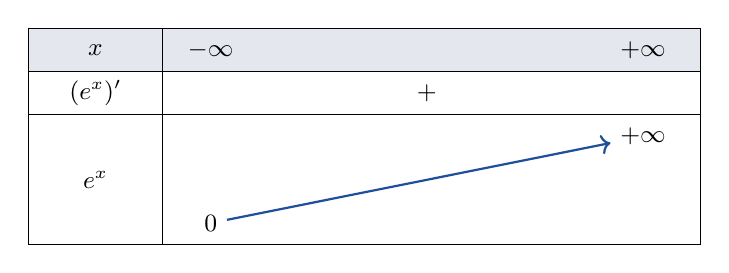
\begin{tikzpicture}[x=1.22cm,y=0.55cm,font=\small]
\fill[cSec!12] (0,0) rectangle (7,-1);
\draw (0,0) rectangle (7,-5); \draw (0,-1)--(7,-1); \draw (0,-2)--(7,-2); \draw (1.4,0)--(1.4,-5);
\node at (0.7,-0.5){$x$}; \node at (0.7,-1.5){$(e^x)^{\prime}$}; \node at (0.7,-3.5){$e^x$};
\node at (1.9,-0.5){$-\infty$}; \node at (6.4,-0.5){$+\infty$}; \node at (4.15,-1.5){$+$};
\node (a) at (1.9,-4.5){$0$}; \node (c) at (6.4,-2.5){$+\infty$}; \draw[->,cDef,thick] (a)--(c);
\end{tikzpicture}\end{LTR}\par \par\smallskip\begin{LTR}\centering \begin{tikzpicture}[x=0.85cm,y=0.85cm,font=\scriptsize]
\draw[->] (-4,0)--(5,0) node[right]{$x$}; \draw[->] (0,-3.5)--(0,5.4) node[above]{$y$};
\draw[gray,densely dotted] (-3,-3)--(5,5) node[below right]{$y=x$};
\draw[cDef,thick,domain=-4:1.65,samples=60] plot (\x,{exp(\x)}) node[left]{$y=e^x$};
\draw[cRem!80!black,thick,domain=0.03:5,samples=80] plot (\x,{ln(\x)}) node[above]{$y=\ln x$};
\draw[cThm,dashed] (-3.5,-2.5)--(2,3) node[right]{$y=x+1$};
\node[left] at (0,1){$1$}; \node[below] at (1,0){$1$};
\end{tikzpicture}\end{LTR}\par }{}{}
\Row{}{%
\Lab{cThm!80!black}{حذار}\ $e^{a+b}\neq e^a+e^b$.}{}{}
\Row{التقويم}{%
\Lab{cMeth}{تمرين تطبيقي}\par\textbf{(1)} بسّط: $A=\dfrac{e^{3x}\times e^{-x}}{e^{x+1}}$.\par\textbf{(2)} احسب: $B=e^{2\ln3}$.\par\textbf{(3)} احسب مشتقة $f(x)=xe^x$.}{25 د}{تقويم فردي.}
\Row{}{%
\Lab{cEx}{حل التمرين التطبيقي}\par\textbf{(1)} $A=\dfrac{e^{3x-x}}{e^{x+1}}=e^{2x-(x+1)}=\RR{e^{x-1}}$.\par\textbf{(2)} $B=e^{\ln(3^2)}=e^{\ln9}=\RR{9}$.\par\textbf{(3)} $f^{\prime}(x)=1\times e^x+x\times e^x=\RR{(x+1)e^x}$.\par\textbf{واجب منزلي:} تمارين من باب الدالة الأسية.\par\smallskip\textbf{ملاحظات حول سير الحصة:} \dotfill}{}{}
\end{Sayr}
\newpage
\ModhHead{35}{3 ت ا}{تحليل}{الدالة الأسية}{02 سا}{حل معادلات ومتراجحات تتضمن أسيات}%
{\begin{itemize}\item خواص الدالة الأسية و $\ln$.\end{itemize}}%
{\begin{itemize}\item حل معادلات ومتراجحات تتضمن $e^x$.\end{itemize}}%
{المنهاج ، الكتاب المدرسي ، الآلة الحاسبة العلمية والبيانية.}
\begin{Sayr}
\Row{مرحلة الانطلاق}{%
\textbf{التهيئة النفسية:} حل: $e^x=3$. وماذا عن $e^x=-1$ ؟}{10 د}{سؤال.}
\Row{التشخيص والاكتشاف}{%
\Lab{cEx}{نشاط 02}\par\textbf{(1)} حل في $\mathbb R$ المعادلة $e^x=3$.\par\textbf{(2)} هل للمعادلة $e^x=-1$ حلول؟}{35 د}{متغير مساعد.}
\Row{}{%
\Lab{cDef}{مناقشة النشاط}\par\textbf{(1)} $e^x=3$ تكافئ $x=\ln3$: $\RR{S=\{\ln3\}}$.\par\textbf{(2)} $e^x>0$ دائماً ، إذن المعادلة \RR{مستحيلة}: $S=\varnothing$.}{}{}
\Row{بناء المعارف}{%
\Lab{cThm}{خاصية}\par\textbf{(1)} $e^a=e^b$ تكافئ $\RR{a=b}$ ؛ $e^a<e^b$ تكافئ $\RR{a<b}$.\par\textbf{(2)} من أجل $k>0$: $e^x=k$ تكافئ $\RR{x=\ln k}$.}{50 د}{التحقق بالآلة الحاسبة.}
\Row{}{%
\Lab{cEx}{مثال 1}\ $e^{2x-1}=1$ تكافئ $e^{2x-1}=e^0$ ، أي $2x-1=0$: $\RR{x=\dfrac12}$.}{}{}
\Row{}{%
\Lab{cEx}{مثال 2}\ $e^{x+1}>e^{3-x}$ تكافئ $x+1>3-x$ ، أي $2x>2$: $\RR{S=]1;+\infty[}$.}{}{}
\Row{}{%
\Lab{cEx}{مثال 3}\ $e^{2x}-3e^x+2=0$: نضع $X=e^x>0$: $X^2-3X+2=0$ ، $(X-1)(X-2)=0$ ، $X=1$ أو $X=2$.\par $e^x=1$ معناه $x=0$ ؛ $e^x=2$ معناه $x=\ln2$: $\RR{S=\{0;\ln2\}}$.}{}{}
\Row{}{%
\Lab{cThm!80!black}{حذار}\ مع المتغير المساعد نرفض الحلول $X\leqslant0$.}{}{}
\Row{التقويم}{%
\Lab{cMeth}{تمرين تطبيقي}\par\textbf{(1)} حل في $\mathbb R$: $e^{2x}-e^x-6=0$.\par\textbf{(2)} حل في $\mathbb R$: $e^{3x-2}\leqslant1$.}{25 د}{تقويم فردي.}
\Row{}{%
\Lab{cEx}{حل التمرين التطبيقي}\par\textbf{(1)} $X=e^x>0$: $X^2-X-6=0$ ، $(X-3)(X+2)=0$ ، $X=3$ أو $X=-2$ (مرفوض). $e^x=3$: $\RR{S=\{\ln3\}}$.\par\textbf{(2)} $e^{3x-2}\leqslant e^0$ تكافئ $3x-2\leqslant0$: $\RR{S=\left]-\infty;\tfrac23\right]}$.\par\textbf{واجب منزلي:} تمارين من باب الدالة الأسية.\par\smallskip\textbf{ملاحظات حول سير الحصة:} \dotfill}{}{}
\end{Sayr}
\newpage
\ModhHead{36}{3 ت ا}{تحليل}{الدالة الأسية}{02 سا}{النهايات الشهيرة والتزايد المقارن ، دوال من الشكل $e^u$}%
{\begin{itemize}\item دراسة الدالة الأسية.\end{itemize}}%
{\begin{itemize}\item معرفة النهايات الشهيرة والتزايد المقارن.\item دراسة دوال من الشكل $e^u$.\end{itemize}}%
{المنهاج ، الكتاب المدرسي ، الآلة الحاسبة العلمية والبيانية.}
\begin{Sayr}
\Row{مرحلة الانطلاق}{%
\textbf{التهيئة النفسية:} أيها «أسرع» عند $+\infty$: $\ln x$ ، $x^2$ أم $e^x$ ؟}{10 د}{الحاسبة البيانية.}
\Row{التشخيص والاكتشاف}{%
\Lab{cEx}{نشاط 03}\par\textbf{(1)} احسب بالآلة الحاسبة $\ln10$ ، $10^2$ ، $e^{10}$.\par\textbf{(2)} رتّب الدوال حسب سرعة تزايدها.}{35 د}{جدول قيم.}
\Row{}{%
\Lab{cDef}{مناقشة النشاط}\par\textbf{(1)} $\ln10\approx2{,}3$ ؛ $10^2=100$ ؛ $e^{10}\approx22026$.\par\textbf{(2)} عند $+\infty$: \RR{الأسية} \RR{تتفوق} \RR{على} \RR{«القوة»} \RR{،} \RR{و«القوة»} \RR{تتفوق} \RR{على} \RR{اللوغاريتم}.}{}{}
\Row{بناء المعارف}{%
\Lab{cThm}{نهايات شهيرة (تُقبل)}\ ($n$ طبيعي غير معدوم):\par\textbf{(1)} $\RR{\lim\limits_{x\to +\infty}\dfrac{e^x}{x^n}=+\infty}$.\par\textbf{(2)} $\RR{\lim\limits_{x\to +\infty}x^ne^{-x}=0}$.\par\textbf{(3)} $\RR{\lim\limits_{x\to -\infty}xe^x=0}$.}{50 د}{جدول التغيرات.}
\Row{}{%
\Lab{cThm}{الدالة $e^u$}\ $\RR{\left(e^u\right)^{\prime}=u^{\prime}e^u}$: لـ $e^u$ نفس اتجاه تغير $u$ ؛ ودالة أصلية لـ $u^{\prime}e^u$ هي $e^u$.}{}{}
\Row{}{%
\Lab{cEx}{مثال 1}\ $\lim\limits_{x\to +\infty}(e^x-x)=\lim\limits_{x\to +\infty}x\left(\dfrac{e^x}x-1\right)=+\infty\times(+\infty)=\RR{+\infty}$.}{}{}
\Row{}{%
\Lab{cEx}{مثال 2}\ $f(x)=xe^{-x}$:\par\textbf{(1)} $f^{\prime}(x)=e^{-x}+x\times(-e^{-x})=\RR{(1-x)e^{-x}}$ ، إشارتها من إشارة $1-x$.\par\textbf{(2)} $\lim\limits_{x\to -\infty}f(x)=-\infty\times(+\infty)=\RR{-\infty}$ ؛ $\lim\limits_{x\to +\infty}f(x)=\RR{0}$ (نهاية شهيرة).\par\textbf{(3)} $f(1)=e^{-1}=\dfrac1e$:\par\smallskip\begin{LTR}\centering 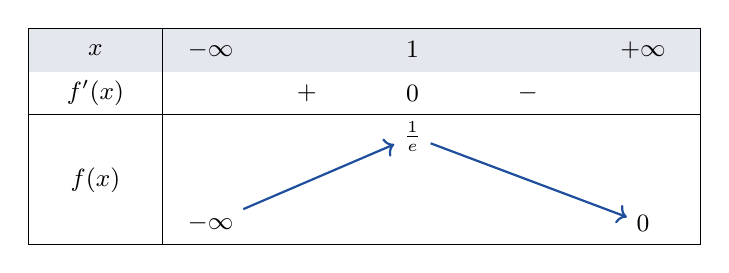
\begin{tikzpicture}[x=1.22cm,y=0.55cm,font=\small]
\draw (0,0) rectangle (7,-5); \draw (0,-1)--(7,-1); \draw (0,-2)--(7,-2); \draw (1.4,0)--(1.4,-5);
\fill[cSec!12] (0,0) rectangle (7,-1); \draw (0,0) rectangle (7,-5); \draw (1.4,0)--(1.4,-5);
\node at (0.7,-0.5){$x$}; \node at (0.7,-1.5){$f^{\prime}(x)$}; \node at (0.7,-3.5){$f(x)$};
\node at (1.9,-0.5){$-\infty$}; \node at (4,-0.5){$1$}; \node at (6.4,-0.5){$+\infty$};
\node at (2.9,-1.5){$+$}; \node at (4,-1.5){$0$}; \node at (5.2,-1.5){$-$};
\node (a) at (1.9,-4.5){$-\infty$}; \node (b) at (4,-2.5){$\frac1e$}; \node (c) at (6.4,-4.5){$0$};
\draw[->,cDef,thick] (a)--(b); \draw[->,cDef,thick] (b)--(c);
\end{tikzpicture}\end{LTR}\par }{}{}
\Row{}{%
\Lab{cThm!80!black}{حذار}\ $e^{-x}>0$: إشارة $f^{\prime}$ هي إشارة العامل الآخر.}{}{}
\Row{التقويم}{%
\Lab{cMeth}{تمرين تطبيقي}\par $g(x)=e^{-x^2+2x}$.\par\textbf{(1)} احسب $g^{\prime}(x)$.\par\textbf{(2)} احسب نهايتي $g$ عند $\pm\infty$.\par\textbf{(3)} شكّل جدول تغيرات $g$.}{25 د}{تقويم فردي.}
\Row{}{%
\Lab{cEx}{حل التمرين التطبيقي}\par\textbf{(1)} $u(x)=-x^2+2x$ ، $u^{\prime}(x)=-2x+2$: $\RR{g^{\prime}(x)=(-2x+2)e^{-x^2+2x}}$.\par\textbf{(2)} $-x^2+2x\to-\infty$ عند $\pm\infty$ ، و $\lim\limits_{X\to-\infty}e^X=0$: $\RR{\lim\limits_{x\to \pm\infty}g(x)=0}$.\par\textbf{(3)} $g(1)=e^{1}=e$:\par\smallskip\begin{LTR}\centering 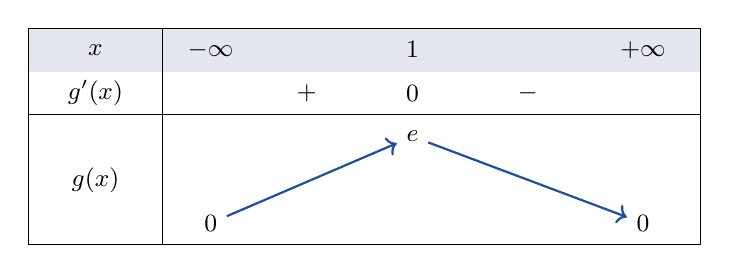
\begin{tikzpicture}[x=1.22cm,y=0.55cm,font=\small]
\draw (0,0) rectangle (7,-5); \draw (0,-1)--(7,-1); \draw (0,-2)--(7,-2); \draw (1.4,0)--(1.4,-5);
\fill[cSec!12] (0,0) rectangle (7,-1); \draw (0,0) rectangle (7,-5); \draw (1.4,0)--(1.4,-5);
\node at (0.7,-0.5){$x$}; \node at (0.7,-1.5){$g^{\prime}(x)$}; \node at (0.7,-3.5){$g(x)$};
\node at (1.9,-0.5){$-\infty$}; \node at (4,-0.5){$1$}; \node at (6.4,-0.5){$+\infty$};
\node at (2.9,-1.5){$+$}; \node at (4,-1.5){$0$}; \node at (5.2,-1.5){$-$};
\node (a) at (1.9,-4.5){$0$}; \node (b) at (4,-2.5){$e$}; \node (c) at (6.4,-4.5){$0$};
\draw[->,cDef,thick] (a)--(b); \draw[->,cDef,thick] (b)--(c);
\end{tikzpicture}\end{LTR}\par \par\textbf{واجب منزلي:} تمارين من باب الدالة الأسية.\par\smallskip\textbf{ملاحظات حول سير الحصة:} \dotfill}{}{}
\end{Sayr}
\newpage
\ModhHead{37}{3 ت ا}{تحليل}{الدالة الأسية}{02 سا}{الدالة الأسية ذات الأساس $a$ ، الدوال القوى}%
{\begin{itemize}\item الدالتان $\ln$ و $\exp$.\end{itemize}}%
{\begin{itemize}\item تعريف $a^x=e^{x\ln a}$ ودراسة اتجاه تغيرها ، والدوال القوى.\end{itemize}}%
{المنهاج ، الكتاب المدرسي ، الآلة الحاسبة العلمية والبيانية.}
\begin{Sayr}
\Row{مرحلة الانطلاق}{%
\textbf{التهيئة النفسية:} آلة ثمنها $500000$ DA تفقد $20\%$ من قيمتها كل سنة: متى تصبح قيمتها أقل من $100000$ DA ؟}{10 د}{وضعية اقتصادية.}
\Row{التشخيص والاكتشاف}{%
\Lab{cEx}{نشاط 04}\par\textbf{(1)} عبّر عن قيمة الآلة $V(t)$ بعد $t$ سنة.\par\textbf{(2)} حل المتراجحة $V(t)<100000$.}{35 د}{الآلة الحاسبة.}
\Row{}{%
\Lab{cDef}{مناقشة النشاط}\par\textbf{(1)} نقصان $20\%$ يعني الضرب في $0{,}8$: $\RR{V(t)=500000\times0{,}8^t}$.\par\textbf{(2)} $0{,}8^t<0{,}2$ ، نطبق $\ln$: $t\ln0{,}8<\ln0{,}2$ ، و $\ln0{,}8<0$ فيتغير اتجاه المتراجحة: $t>\dfrac{\ln0{,}2}{\ln0{,}8}\approx7{,}21$: \RR{بعد} \RR{$8$} \RR{سنوات}.}{}{}
\Row{بناء المعارف}{%
\Lab{cDef}{تعريف}\ من أجل $a>0$: $\RR{a^x=e^{x\ln a}}$ ($x$ حقيقي). \textbf{الدالة القوة}: $\RR{x^\alpha=e^{\alpha\ln x}}$ ($x>0$).}{50 د}{المقارنة بين $a>1$ و $a<1$.}
\Row{}{%
\Lab{cThm}{خاصية}\par\textbf{(1)} $\RR{\left(a^x\right)^{\prime}=\ln a\times a^x}$: متزايدة تماماً إذا $a>1$ ، متناقصة تماماً إذا $0<a<1$.\par\textbf{(2)} $\RR{\left(x^\alpha\right)^{\prime}=\alpha x^{\alpha-1}}$ ؛ $x^{\frac12}=\sqrt x$.}{}{}
\Row{}{%
\Lab{cEx}{مثال}\par\textbf{(1)} $2^x=10$ تكافئ $x\ln2=\ln10$: $x=\dfrac{\ln10}{\ln2}\approx\RR{3{,}32}$.\par\textbf{(2)} $\left(2^x\right)^{\prime}=\RR{\ln2\times2^x}$.\par\textbf{(3)} $0<0{,}5<1$: $0{,}5^x$ \RR{متناقصة} \RR{تماماً}.}{}{}
\Row{}{%
\Lab{cThm!80!black}{حذار}\ القسمة على $\ln a<0$ (لما $0<a<1$) تقلب اتجاه المتراجحة.}{}{}
\Row{التقويم}{%
\Lab{cMeth}{تمرين تطبيقي}\par\textbf{(1)} حل في $\mathbb R$: $1{,}5^x\geqslant100$.\par\textbf{(2)} احسب مشتقة $f(x)=x^{1{,}5}$ على $]0;+\infty[$.}{25 د}{تقويم فردي.}
\Row{}{%
\Lab{cEx}{حل التمرين التطبيقي}\par\textbf{(1)} $x\ln1{,}5\geqslant\ln100$ ، و $\ln1{,}5>0$: $x\geqslant\dfrac{\ln100}{\ln1{,}5}\approx\RR{11{,}36}$.\par\textbf{(2)} $f^{\prime}(x)=1{,}5\,x^{0{,}5}=\RR{1{,}5\sqrt x}$.\par\textbf{واجب منزلي:} تمارين من باب الدالة الأسية.\par\smallskip\textbf{ملاحظات حول سير الحصة:} \dotfill}{}{}
\end{Sayr}
\newpage
\ModhHead{38}{3 ت ا}{تحليل}{الدالة الأسية}{02 سا}{حل مشكلات متعلقة بإيداع أو تسديد}%
{\begin{itemize}\item المتتاليات الهندسية ، $\ln$ ، $a^x$.\end{itemize}}%
{\begin{itemize}\item حل مشكلات إيداع وتسديد تتدخل فيها اللوغاريتمات أو الأسيات.\end{itemize}}%
{المنهاج ، الكتاب المدرسي ، الآلة الحاسبة العلمية والبيانية.}
\begin{Sayr}
\Row{مرحلة الانطلاق}{%
\textbf{التهيئة النفسية:} مؤسسة تقترض $1000000$ DA بنسبة $5\%$ وتسدد بأقساط سنوية ثابتة على $10$ سنوات: ما قيمة القسط؟}{10 د}{وضعية مالية.}
\Row{التشخيص والاكتشاف}{%
\Lab{cEx}{مشكلة (إيداع)}\ إيداع $200000$ DA بفائدة مركبة $4\%$ سنوياً.\par\textbf{(1)} عبّر عن الرصيد $C_n$ بعد $n$ سنة.\par\textbf{(2)} بعد كم سنة يتضاعف الرصيد؟}{35 د}{ربط بالمتتاليات.}
\Row{}{%
\Lab{cDef}{مناقشة النشاط}\par\textbf{(1)} متتالية هندسية أساسها $1{,}04$: $\RR{C_n=200000\times1{,}04^n}$.\par\textbf{(2)} $1{,}04^n\geqslant2$ ، $n\ln1{,}04\geqslant\ln2$ ، $n\geqslant\dfrac{\ln2}{\ln1{,}04}\approx17{,}67$: \RR{بعد} \RR{$18$} \RR{سنة}.}{}{}
\Row{بناء المعارف}{%
\Lab{cMeth}{طريقة}\ نكتب الحد العام (هندسي غالباً) ، ثم نحل متراجحة أسية بتطبيق $\ln$.}{50 د}{الآلة الحاسبة.}
\Row{}{%
\Lab{cThm}{التسديد بأقساط ثابتة (تُقبل)}\ قرض $C$ بنسبة $t$ يُسدد بـ $n$ قسطاً سنوياً ثابتاً: $\RR{a=\dfrac{C\,t}{1-(1+t)^{-n}}}$.}{}{}
\Row{}{%
\Lab{cEx}{مثال}\ $C=1000000$ ، $t=0{,}05$ ، $n=10$: $a=\dfrac{1000000\times0{,}05}{1-1{,}05^{-10}}=\dfrac{50000}{1-0{,}6139}\approx\RR{129505}$ DA.}{}{}
\Row{}{%
\Lab{cThm!80!black}{حذار}\ $n$ عدد طبيعي: نأخذ أول عدد طبيعي يحقق المتراجحة.}{}{}
\Row{التقويم}{%
\Lab{cMeth}{تمرين تطبيقي}\par إيداع $150000$ DA بفائدة مركبة $3{,}5\%$ سنوياً.\par\textbf{(1)} عبّر عن الرصيد بعد $n$ سنة.\par\textbf{(2)} بعد كم سنة يتجاوز الرصيد $200000$ DA ؟}{25 د}{تقويم فردي.}
\Row{}{%
\Lab{cEx}{حل التمرين التطبيقي}\par\textbf{(1)} $\RR{C_n=150000\times1{,}035^n}$.\par\textbf{(2)} $1{,}035^n\geqslant\dfrac{200000}{150000}=\dfrac43$ ، $n\geqslant\dfrac{\ln\frac43}{\ln1{,}035}\approx8{,}36$: \RR{بعد} \RR{$9$} \RR{سنوات}.\par\textbf{واجب منزلي:} مسائل من صفحة 143 إلى 147.\par\smallskip\textbf{ملاحظات حول سير الحصة:} \dotfill}{}{}
\end{Sayr}
\newpage
\ModhHead{39}{3 ت ا}{تحليل}{الدالة الأسية}{02 سا}{حل مسائل حول دراسة دوال لوغاريتمية وأسية}%
{\begin{itemize}\item دراسة $\ln$ و $\exp$ ، النهايات الشهيرة.\end{itemize}}%
{\begin{itemize}\item دراسة دالة لوغاريتمية أو أسية كاملة وتمثيلها البياني.\end{itemize}}%
{المنهاج ، الكتاب المدرسي ، الآلة الحاسبة العلمية والبيانية. ورق ميليمتري.}
\begin{Sayr}
\Row{مرحلة الانطلاق}{%
\textbf{التهيئة النفسية:} ما خطوات دراسة دالة؟ وما الجديد مع $\ln$ و $\exp$ ؟}{10 د}{سؤال تلخيصي.}
\Row{التشخيص والاكتشاف}{%
\Lab{cEx}{مسألة}\ $f(x)=\dfrac{\ln x}x$ على $]0;+\infty[$.\par\textbf{(1)} احسب نهايتي $f$ عند $0^{+}$ و $+\infty$ ، واستنتج المقاربات.\par\textbf{(2)} بيّن أن $f^{\prime}(x)=\dfrac{1-\ln x}{x^2}$ ، وشكّل جدول التغيرات.\par\textbf{(3)} عيّن نقطة تقاطع $(C_f)$ مع محور الفواصل وارسم $(C_f)$.}{35 د}{عمل بالأفواج.}
\Row{}{%
\Lab{cDef}{مناقشة النشاط}\par\textbf{(1)} $\ln x\to-\infty$ و $\dfrac1x\to+\infty$: $\RR{\lim\limits_{x\to 0^{+}}f(x)=-\infty}$ (محور التراتيب مقارب) ؛ $\RR{\lim\limits_{x\to +\infty}f(x)=0}$ (نهاية شهيرة ، محور الفواصل مقارب).}{}{}
\Row{بناء المعارف}{%
\Lab{cEx}{الدراسة}\par\textbf{(2)} $f^{\prime}(x)=\dfrac{\frac1x\times x-\ln x\times1}{x^2}=\RR{\dfrac{1-\ln x}{x^2}}$ ، إشارتها من إشارة $1-\ln x$: موجبة لما $x<e$. و $f(e)=\dfrac1e$:\par\smallskip\begin{LTR}\centering 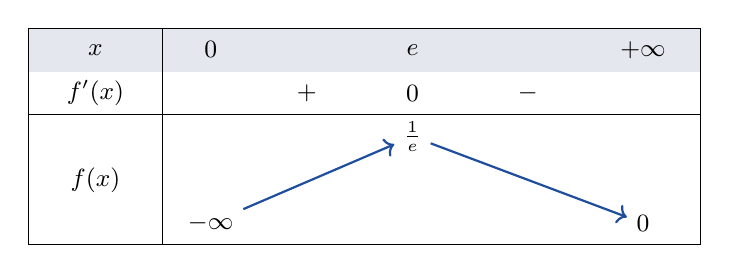
\begin{tikzpicture}[x=1.22cm,y=0.55cm,font=\small]
\draw (0,0) rectangle (7,-5); \draw (0,-1)--(7,-1); \draw (0,-2)--(7,-2); \draw (1.4,0)--(1.4,-5);
\fill[cSec!12] (0,0) rectangle (7,-1); \draw (0,0) rectangle (7,-5); \draw (1.4,0)--(1.4,-5);
\node at (0.7,-0.5){$x$}; \node at (0.7,-1.5){$f^{\prime}(x)$}; \node at (0.7,-3.5){$f(x)$};
\node at (1.9,-0.5){$0$}; \node at (4,-0.5){$e$}; \node at (6.4,-0.5){$+\infty$};
\node at (2.9,-1.5){$+$}; \node at (4,-1.5){$0$}; \node at (5.2,-1.5){$-$};
\node (a) at (1.9,-4.5){$-\infty$}; \node (b) at (4,-2.5){$\frac1e$}; \node (c) at (6.4,-4.5){$0$};
\draw[->,cDef,thick] (a)--(b); \draw[->,cDef,thick] (b)--(c);
\end{tikzpicture}\end{LTR}\par \par\textbf{(3)} $f(x)=0$ معناه $\ln x=0$ أي $x=1$: النقطة $\RR{(1;0)}$.\par\smallskip\begin{LTR}\centering \begin{tikzpicture}[x=0.75cm,y=1.6cm,font=\scriptsize]
\draw[->] (-0.4,0)--(10.5,0) node[right]{$x$}; \draw[->] (0,-1.6)--(0,0.9) node[above]{$y$};
\draw[cDef,thick,domain=0.42:10.3,samples=100] plot (\x,{ln(\x)/\x}) node[above]{$C_f$};
\draw[densely dotted] (2.718,0)--(2.718,0.368)--(0,0.368); \node[left] at (0,0.368){$\frac1e$}; \node[below] at (2.718,0){$e$}; \node[below] at (1,0){$1$};
\end{tikzpicture}\end{LTR}\par }{50 د}{رسم بالحاسبة للتحقق.}
\Row{}{%
\Lab{cThm!80!black}{حذار}\ إشارة $\ln x$: سالبة على $]0;1[$ ، موجبة على $]1;+\infty[$.}{}{}
\Row{التقويم}{%
\Lab{cMeth}{تمرين تطبيقي}\par $g(x)=(x-1)e^x$ على $\mathbb R$.\par\textbf{(1)} احسب نهايتي $g$ عند $\pm\infty$.\par\textbf{(2)} احسب $g^{\prime}(x)$ وشكّل جدول التغيرات.}{25 د}{نهاية المحور: فرض أو معالجة بيداغوجية.}
\Row{}{%
\Lab{cEx}{حل التمرين التطبيقي}\par\textbf{(1)} $\lim\limits_{x\to -\infty}g(x)=\lim\limits_{x\to -\infty}\left(xe^x-e^x\right)=0-0=\RR{0}$ ؛ $\lim\limits_{x\to +\infty}g(x)=\RR{+\infty}$.\par\textbf{(2)} $g^{\prime}(x)=e^x+(x-1)e^x=\RR{xe^x}$ ، إشارتها من إشارة $x$ ؛ $g(0)=-1$:\par\smallskip\begin{LTR}\centering 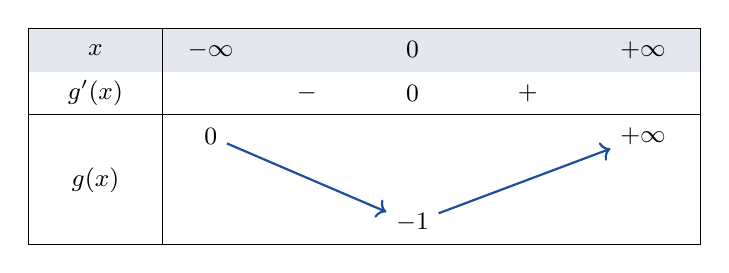
\begin{tikzpicture}[x=1.22cm,y=0.55cm,font=\small]
\draw (0,0) rectangle (7,-5); \draw (0,-1)--(7,-1); \draw (0,-2)--(7,-2); \draw (1.4,0)--(1.4,-5);
\fill[cSec!12] (0,0) rectangle (7,-1); \draw (0,0) rectangle (7,-5); \draw (1.4,0)--(1.4,-5);
\node at (0.7,-0.5){$x$}; \node at (0.7,-1.5){$g^{\prime}(x)$}; \node at (0.7,-3.5){$g(x)$};
\node at (1.9,-0.5){$-\infty$}; \node at (4,-0.5){$0$}; \node at (6.4,-0.5){$+\infty$};
\node at (2.9,-1.5){$-$}; \node at (4,-1.5){$0$}; \node at (5.2,-1.5){$+$};
\node (a) at (1.9,-2.5){$0$}; \node (b) at (4,-4.5){$-1$}; \node (c) at (6.4,-2.5){$+\infty$};
\draw[->,cDef,thick] (a)--(b); \draw[->,cDef,thick] (b)--(c);
\end{tikzpicture}\end{LTR}\par \par\textbf{واجب منزلي:} مسائل من صفحة 143 إلى 147.\par\smallskip\textbf{ملاحظات حول سير الحصة:} \dotfill}{}{}
\end{Sayr}
\end{document}
